\section{Modellazione dei programmi}
L'obiettivo dell'analisi statica è certificare che un programma sia sicuro
rispetto a determinati errori, come ad esempio la divisione per zero.

\subsection{Poset nell'analisi statica}

L'idea fondamentale è calcolare i possibili valori che una variabile può
assumere in ogni punto del programma, considerando tutte le possibili
esecuzioni.
Per fare questo è possibile utilizzare i reticoli (Definizione
\Cref{def:lattice}).

\begin{esempio}{Esempio di reticolo su un programma}{}
Considerando il programma seguente:

\begin{verbatim}
1: i = read ();
2 if ( i != 0 )
3   j = 5 / i ;
4 else
5   j = 0;
6 return;
\end{verbatim}

e definendo il reticolo dei valori interi come $\langle
\mathcal{P}(\mathbb{Z}), \subseteq, \cup, \cap \rangle$ è possibile
calcolare i possibili valori delle variabili $i$ e $j$ in ogni punto
del programma.

\medskip

\begin{center}
\begin{tabular}{|c|l|}
  \hline
  \textbf{Program point} & \textbf{Valori} \\
  \hline
  \hline
  1 & $i = \{\}, \ j = \{\}$ \\
  \hline
  2 & $i = \mathbb{Z}, \ j = \{\}$ \\
  \hline
  3 & $i = \mathbb{Z} \setminus \{0\}, \ j = \{5 / i \}$ \\
  \hline
  5 & $i = \{0\}, \ j = \{0\}$ \\
  \hline
  6 & $i = \mathbb{Z}, \ j = \{-5, -2, -1, 0, 1, 2, 5 \}$ \\
  \hline
\end{tabular}
\end{center}

Per ottenere i valori di $j$ al punto $6$, è stato necessario calcolare
l'unione dei valori di $j$ provenienti dai punti $3$ e $5$, utilizzando
l'operazione di least upper bound (operazione di join, unione insiemistica
in questo caso).

Per ottenere i valori di $i$ al punto $2$, è stato necessario considerare
che la funzione \texttt{read()} può restituire qualsiasi valore intero.
Dopo di che tramite un'operazione di ``filtro'' $filter(i \neq 0)$ è
  possibile restringere i valori di $i$ per entrare nel ramo vero dell'if.
Per il calcolo del punto $3$, invece è stato necessario applicare l'operazione
di intersezione tra i valori di $i$ al punto $2$ e il filtro $filter(x \neq 0)$
per ottenere i valori di $i$ validi per quel ramo.


Ipotizzando che la funzione \texttt{read()} possa restituire valori interi in
$\{ -1, 0, 1 \}$, è possibile riscrivere il codice del programma di esempio
come:
\begin{verbatim}
1: i = {-1, 0, 1} ;
2 if ( i != 0 )
3   j = 5 / i ;
4 else
5   j = 0;
6 return;
\end{verbatim}
Di conseguenza i valori delle variabili in ogni punto del programma
diventano:

\medskip

\begin{center}
\begin{tabular}{|c|l|}
  \hline
  \textbf{Program point} & \textbf{Valori} \\
  \hline
  \hline
  1 & $i = \{\}, \ j = \{\}$ \\
  \hline
  2 & $i = [-1, 1], \ j = \{\}$ \\
  \hline
  3 & $i = [-1, -1] \cup [1, 1], \ j = [ -5, 5 ]$ \\
  \hline
  5 & $i = [0, 0], \ j = [0, 0]$ \\
  \hline
  6 & $i = [-1, 1], \ j = [-5, 5]$ \\
  \hline
\end{tabular}
\end{center}
\end{esempio}


\subsection{Punti fissi}
Quando il programma contiene dei cicli (come \texttt{while}), il numero di
esecuzioni possibili diventa arbitrario o infinito.
Per analizzare queste strutture, utilizziamo il concetto di punto fisso
(Definizione \Cref{def:fixpoint}).
L'analisi procede iterativamente accumulando informazioni
(tramite il Join $\cup$) finché lo stato non si stabilizza.

\begin{esempio}{Analisi di un ciclo su dominio infinito (Non terminazione)}{fixpoint_infinite}

Considerando il programma seguente che presenta un ciclo infinito che
incrementa un contatore:

\begin{verbatim}
1: i = 0;
2: while (?)
3:   i++;
4: ...
\end{verbatim}

Utilizzando il reticolo $\langle \mathcal{P}(\mathbb{Z}), \subseteq, \cup, \cap \rangle$,
è possibile calcolare i valori di $i$ al punto $2$ (l'ingresso del ciclo).
Lo stato al punto $2$ è definito come l'unione del valore iniziale (da 1) e
del valore di ritorno dal ciclo (da 3):
\[ Val(2) = \{0\} \cup (Val(3) + 1) \]

Passo passo:

\medskip

\begin{center}
\renewcommand{\arraystretch}{1.3}
\begin{tabular}{|c|l|l|}
  \hline
  \textbf{Iterazione} & \textbf{Valori al Punto 2} & \textbf{Valori al Punto 3} \\
  \hline
  \hline
  0 & $\emptyset$ & $\emptyset$ \\
  \hline
  1 & $\{0\}$ & $\emptyset$ \\
  \hline
  2 & $\{0\}$ & $\{0\}$ \\
  \hline
  3 & $\{0\} \cup \{0+1\} = \{0, 1\}$ & $\{0\}$ \\
  \hline
  4 & $\{0, 1\}$ & $\{0, 1\}$ \\
  \hline
  5 & $\{0, 1\} \cup \{1+1\} = \{0, 1, 2\}$ & $\{0, 1\}$ \\
  \hline
  \dots & \dots & \dots \\
  \hline
\end{tabular}
\end{center}

Si nota che l'insieme continua a crescere ($ \{0, 1, 2, 3, \dots\} $) e,
poiché il reticolo $\mathcal{P}(\mathbb{Z})$ ha altezza infinita, l'algoritmo
non raggiunge mai un punto fisso in tempo finito.
\end{esempio}

\subsection{IMP}

IMP è un linguaggio imperativo minimale che supporta assegnamenti,
sequenze, condizionali e cicli.

\subsubsection{Sintassi}
La sintassi del linguaggio è definita dalle seguenti produzioni
grammaticali:
\begin{itemize}
    \item \textbf{Espressioni aritmetiche ($e$):}
    \[ e ::= x \mid n \mid e_1 \ op_a \ e_2 \]
    dove $x$ è una variabile, $n \in \mathbb{Z}$ è un intero, e $op_a \in \{+, -, *, \div\}$.

    \item \textbf{Espressioni booleane ($b$):}
    \[ b ::= \text{true} \mid \text{false} \mid \neg b \mid b_1 \ op_b \ b_2 \mid e_1 \ op_c \ e_2 \]
    dove $op_b \in \{\&\&, ||\}$ (logici) e $op_c \in \{==, <, >, \le, \ge\}$ (confronto).

    \item \textbf{Statement ($s$):}
    \[ s ::= x := e ; \mid \textbf{skip} \mid s_1 s_2 \mid \textbf{if}\ b \textbf{then}\ s_1 \textbf{else}\ s_2 \mid \textbf{while}\ b \textbf{do}\ s_1 \]
\end{itemize}


\subsubsection{Semantica concreta}
%TODO

\subsection{Semantica delle tracce}

Per analizzare il comportamento di un programma, è necessario definire cosa
significa ``eseguirlo''. La semantica di traccia modella l'esecuzione
come una sequenza (traiettoria) di stati nel tempo.

\begin{definizione}{Traccia}{trace}
Una traccia $\tau \in X^{\infty}$ è una sequenza di stati che rappresenta una singola
evoluzione del programma. Le tracce possono essere:
\begin{itemize}
    \item \textbf{Finite:} L'esecuzione termina in uno stato finale.
    \item \textbf{Infinite:} L'esecuzione non termina (es. ciclo infinito).
    \item \textbf{Parziali:} Rappresentano un prefisso dell'esecuzione fino a un certo punto intermedio.
\end{itemize}
\end{definizione}


\begin{definizione}{Semantica delle tracce}{trace_semantics}
È possibile modellare la semantica concreta, ovvero l'insieme di tutte le
possibili esecuzioni, utilizzando un reticolo definito come:
\[
\langle \mathcal{P}(X^{\infty}), \subseteq, \cup, \cap \rangle
\]

\begin{figure}[H]
  \centering
  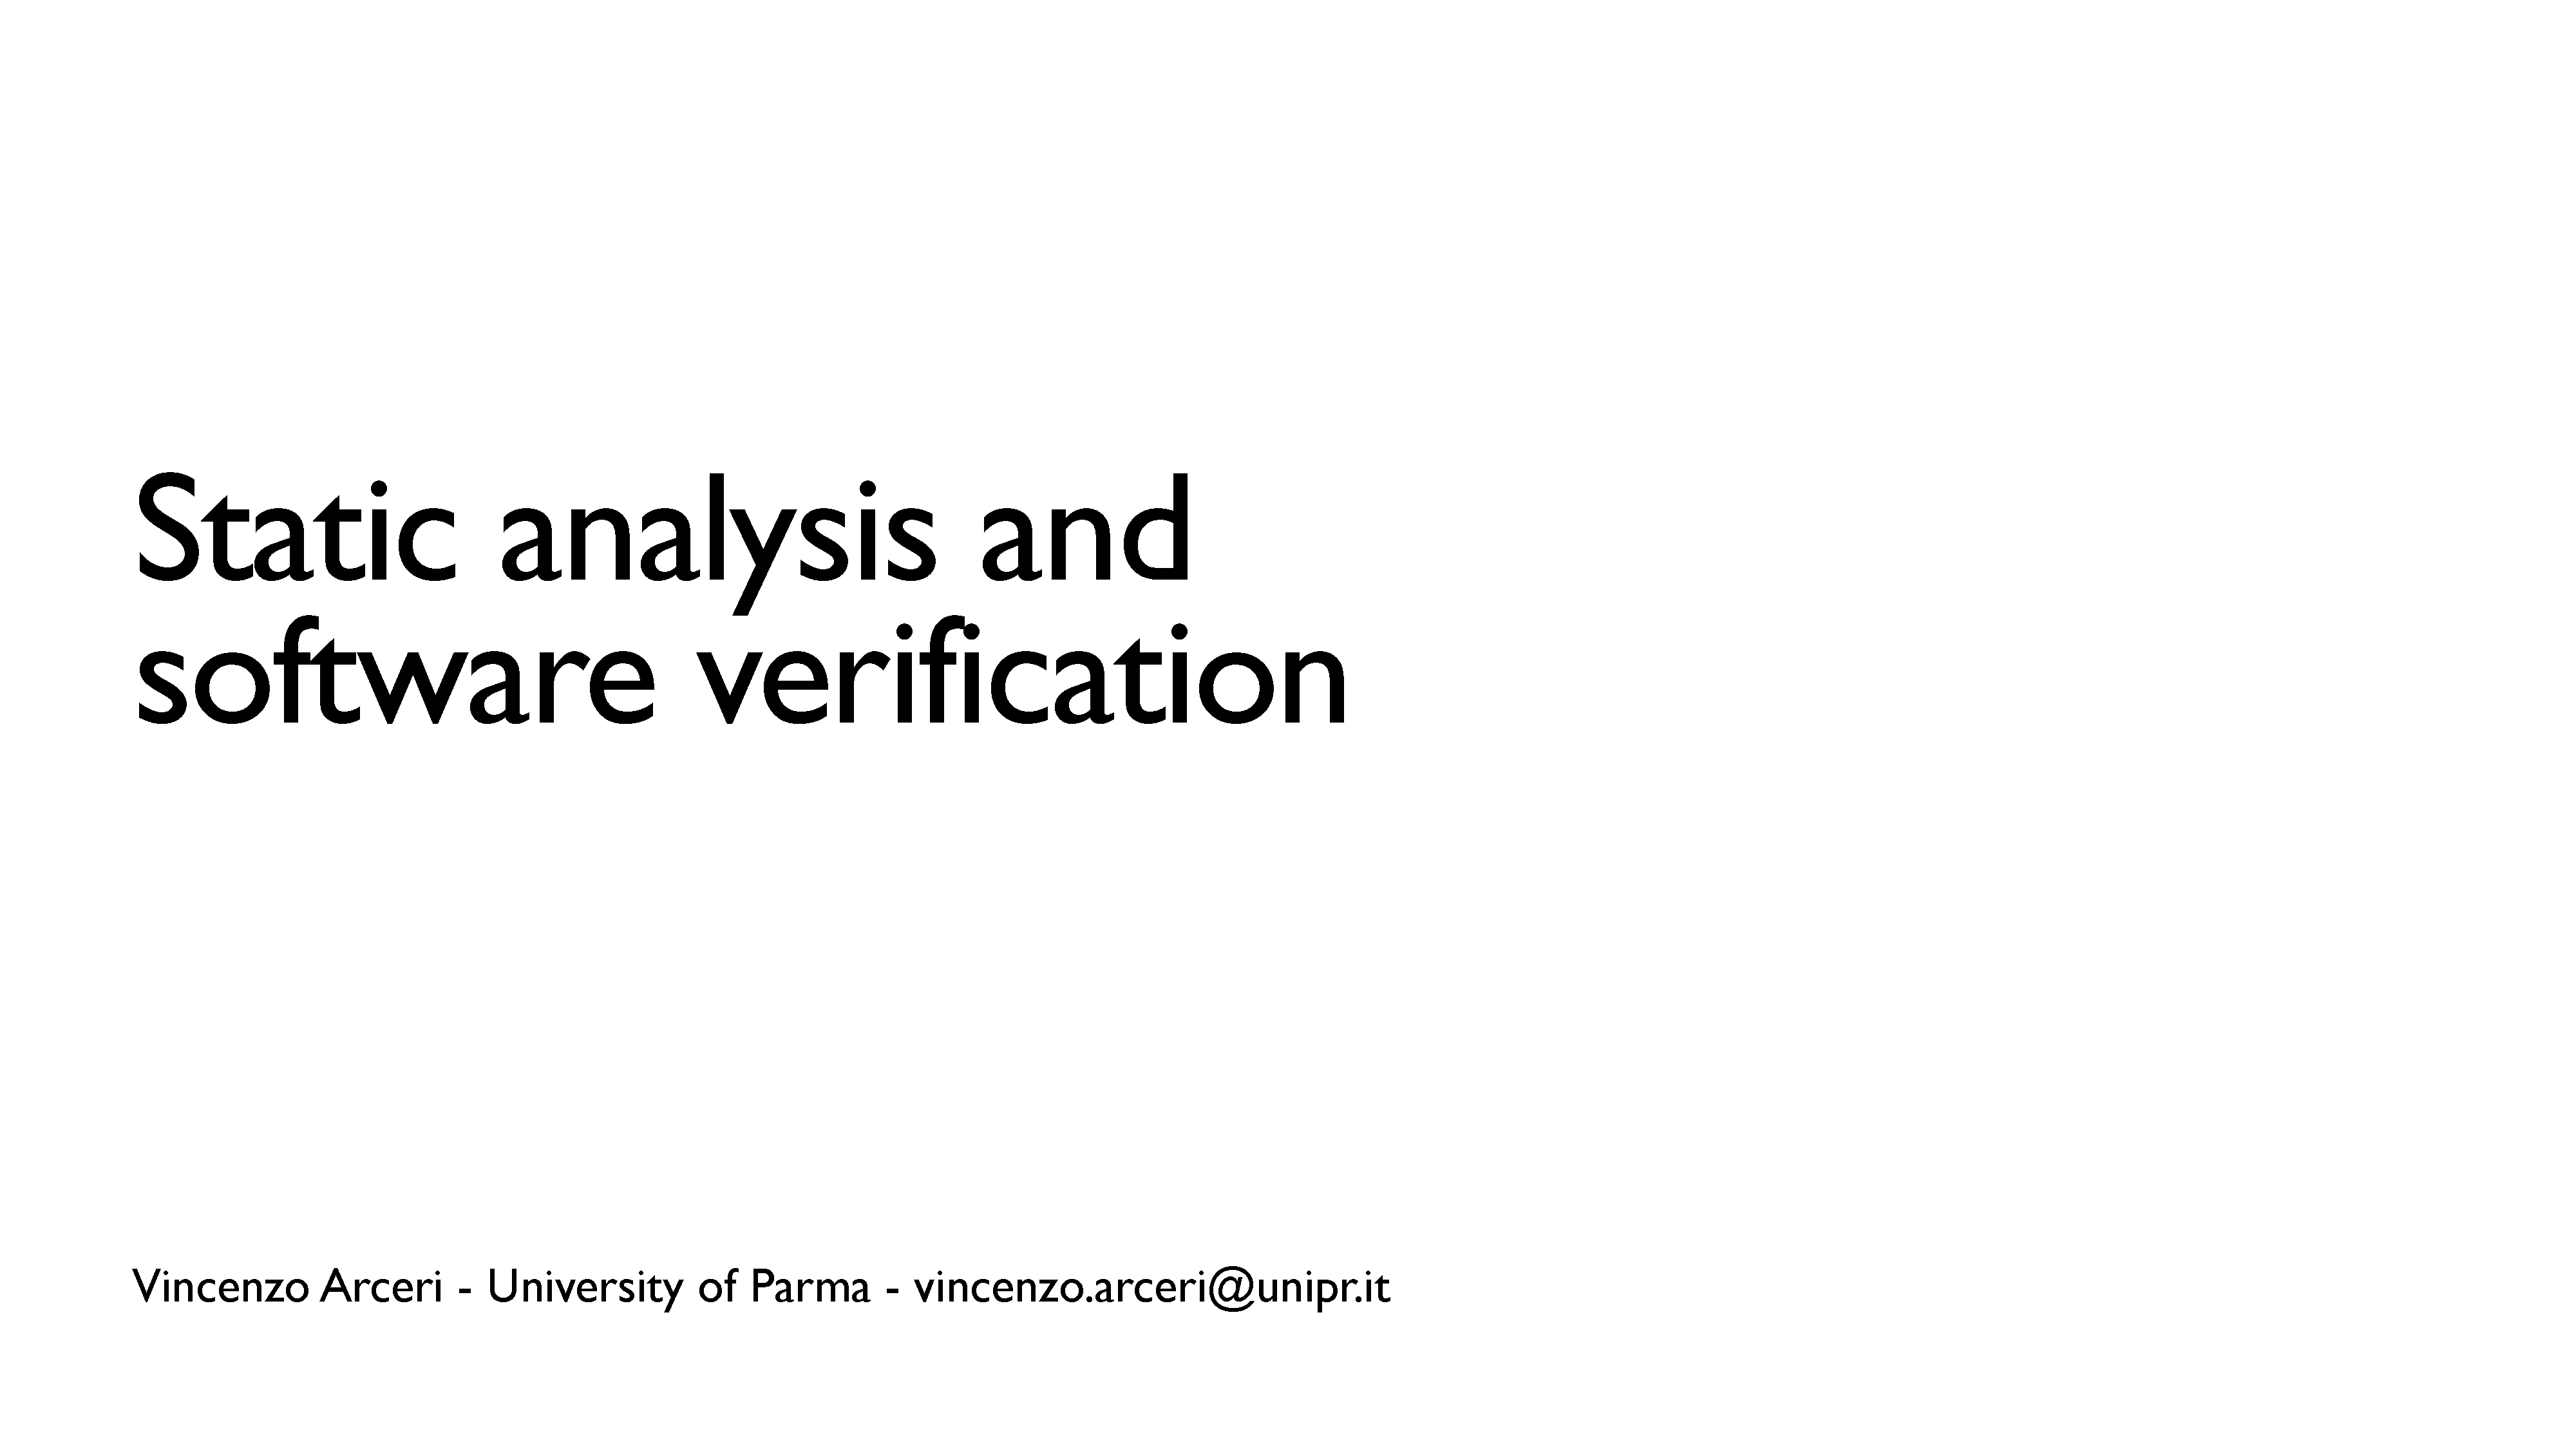
\includegraphics[width=0.6\textwidth]{images/th_03/01.png}
  \caption{L'immagine illustra l'insieme delle tracce di un programma.}
  \label{fig:th_03_01}
\end{figure}

\end{definizione}

\begin{nota}{Calcolo della semantica}{trace_semantics_fixpoint}
La semantica del programma viene calcolata come il least fixpoint (lfp) di
una funzione che costruisce le tracce passo dopo passo:
\begin{enumerate}
    \item Si parte dalle tracce di lunghezza 1 (stati iniziali).
    \item Si applica iterativamente la funzione di transizione per estendere
    le tracce parziali.
    \item Si uniscono ($\cup$) i risultati fino a raggiungere il punto fisso.
\end{enumerate}
Questo processo cattura sia le esecuzioni che terminano, sia quelle che
divergono (loop infiniti).

\end{nota}

\subsection{Calcolo del least fixpoint}

Il calcolo della semantica di un programma $P$ si riduce alla ricerca del
least fixpoint (lfp) della sua funzione semantica $F_P$.

\begin{proposizione}{Procedura Iterativa}{lfp_computation}
Il least fixpoint si calcola iterando la funzione $F_P$ a partire
dall'elemento \textit{bottom} ($\bot$) del reticolo, procedendo dal
``basso verso l'alto'':

\[ lfp(F_P) = \bigsqcup_{n \in \mathbb{N}} F_P^n(\bot) \]

La sequenza delle iterazioni costruisce progressivamente la semantica:
\begin{itemize}
    \item Passo 0: $F^0(\bot) = \bot$ (stato iniziale vuoto o non inizializzato).
    \item Passo 1: $F^1(\bot) = F(\bot)$ (prime esecuzioni parziali, es. stati iniziali).
    \item Passo $k$: $F^k(\bot)$ (insieme delle esecuzioni parziali di lunghezza fino a $k$).
\end{itemize}
Il processo termina quando si raggiunge un punto fisso, ovvero quando
$F^{k+1}(\bot) = F^k(\bot)$.

\begin{figure}[H]
  \centering
  \includegraphics[width=0.6\textwidth]{images/th_03/02.png}
  \caption{L'immagine illustra l'insieme delle tracce finite e infinite
  di un programma, con gli stati iniziali, stati intermedi e stati finali.}
  \label{fig:th_03_02}
\end{figure}

\end{proposizione}

\begin{nota}{Significato delle iterazioni}{partial_executions}
In questo modo, ad ogni passo dell'iterazione otteniamo un insieme di
esecuzioni parziali.
L'unione di tutte queste iterazioni fino al punto fisso ci fornisce la
semantica completa del programma, che include sia le tracce finite che quelle
infinite.
\end{nota}